\chapter{Coupling between India and China: A dynamical hypothesis}

\section{Proposed Mechanism}

	We propose that years of anomalously heavy July-August rainfall over the Himalayan Foothills reflect increased transport of water vapor from the Bay of Bengal. In turn, some of this surplus vapor travels via northeastern India to the southeastern Tibetan Plateau and northern Yunnan Plateau, and onward to the Yangtze Corridor. In \cite{Sampe2010}, a linear baroclinic model (LBM) with prescribed heating over the Yangtze Corridor produced a zonal band of ascent, as well as anomalous descent to the north and south (Figures 13 and 14 of their paper). We suggest that increased latent heating associated with an increase in water vapor along the Yangtze Corridor may supply a diabatic forcing similar to the Sampe and Xie experiment, and that the resulting vertical velocity anomalies could ultimately generate the tripole pattern of rainfall anomalies over China seen in All-Asia JA EOF1. In months with reduced moisture transport across the Yunnan Plateau, we therefore propose that the decrease in latent heating along the Yangtze Corridor would lead to anomalous local descent and an inverted spatial pattern of rainfall anomalies. We further theorize that the coupling between India and China begins in July, when the onset of monsoon circulation in northern India initiates abundant moisture transport toward the Himalayas and onward to the Yunnan Plateau, and ends by September due to the shift of peak insolation back to the Equator.
	
	The strong dipole of Indian summer rainfall variability, and corresponding shift in moisture transport, may reflect the existence of two stable summer ITCZ positions over India: An oceanic latitude at 5\textdegree N and a continental latitude at 15\textdegree N, as argued in \cite{Gadgil2003}. In turn, the preferred configuration of the ITCZ may be influenced by the state of ENSO and Indian Ocean SST. A full moisture budget equates the \textit{convergence} of moisture transport with the balance of precipitation and evaporation ($P-E$) \citep{Trenberth1991,Chen2014b}. For our purposes, we assume that an additional influx of moisture from the Bay of Bengal must translate to increased precipitation downstream. Also, our subsequent model results suggest that evaporation is a negligible component of the moisture budget during the monsoon.
		
\section{Potential Vorticity and Moist Static Energy}

	The linkage of July-August rainfall anomalies in India and China can be understood in terms of conservation of potential vorticity (PV). The PV of a column of air is given by
	\begin{displaymath}
			PV  \thickapprox \frac{\left(\xi+f\right)}{H}  = \mathrm{ constant}
	\end{displaymath}
	
	where $\xi = \frac{\partial v}{\partial x}-\frac{\partial u}{\partial y}$ is the relative vorticity of the column, $f=2\Omega\mathrm{sin}\phi$ is the planetary vorticity at latitude $\phi$ due to the rotation rate of the Earth $\Omega$, and $H$ is the height of the column. This approximation is valid for a barotropic fluid. In this simple framework, heating acts by stretching a parcel and topography by compressing it. This helps to explain the sensitivity of flow even to low topography, and why moisture does not simply pass over the Arakan Mountains or Ghats.
	
	A moisture parcel propagating northward from the Bay of Bengal cannot overcome the steep topography gradient of the Himalayas (which sharply decreases $H$). Instead, trajectories bifurcate between a westward branch towards Nepal ($\xi > 0$) and eastward forced channel flow between the Himalayas and Arakan Mountains into northeastern India ($\xi < 0$). These two trajectories encounter different topography. To the west, the Himalayas exceed 5 km of altitude, preventing access of moisture to the quasi-desertic Western Tibetan Plateau. To the east, the Himalayas are slightly lower, the slopes are less steep, and river valleys allow access to the high terrain of the eastern Tibetan Plateau and Yunnan Plateau. During monsoon season, moisture is observed to propagate as far as Lhasa and up the Brahmaputra and Zayu river valleys, which run from the Tibetan Plateau's southeastern edge into northeastern India \citep{Gao2011,Yang2011}. Propagation may also be aided by the phenomenon described in \cite{Holton2004} that perturbations in easterly flow are damped whereas westerly flow excursions are amplified due to the gradient of planetary vorticity. Lastly, moist flow upslope may be abetted by surface heating, which should lift isentropes \citep{Molnar1999,Prive2007a}. 
	
	In practice, we lack information about individual parcels. Instead, moist static energy $h$, and in particular the subcloud quantity $h_b$, reveals information about the strength and extent of the monsoon \citep{Prive2007,Prive2007a}. $h$ tracks total potential energy per kilogram of air (units of J kg$^{-1}$ or m$^2$ s$^{-2}$), including latent heating, sensible heating and potential energy:
	\begin{displaymath}
			h= L_v q+c_p T+gz
	\end{displaymath}
		
	$L_v$ is the latent heat of vaporization of water and $c_p$ the specific heat of dry air. In the absence of diabatic heating, this quantity remains conserved. Following \cite{Boos2010}, $h$ is expressed in units of Kelvin by dividing by $c_p$. The resulting quantity can be interpreted as the equivalent temperature the parcel would have at sea level if all moisture was condensed. According to both idealized studies and observation, the maximum of $h_b$ occurs at the northernmost extent of monsoon circulation  \citep{Emanuel1995,Prive2007,Boos2010,Nie2010}. Therefore, if our hypothesis of abundant moisture transport from the Bay of Bengal to northeastern India and onward is correct, we should observe an associated $h_b$ maximum there that also diffuses downstream onto the southern Tibetan Plateau, northern Yunnan Plateau and beyond. The Himalayas amplify the $h_b$ maximum along the Himalayan Foothills both by shielding warm air over India from cold air further north \citep{Boos2010} and by forced wind and moisture convergence. The Arakan Mountains may further induce convergence and strengthen $h_b$ by restricting atmospheric flow into northeastern India to a narrow channel.

\section{Supporting Evidence}

	APHRODITE shows that northeastern India experiences intense summer rainfall of 20 to 30 mm day$^{-1}$ (Figure ~\ref{fig:f21}). Such rates require substantial moisture advection inland. Several past studies demonstrate this transport. As previously mentioned in sections 3b and 6d, studies of $\delta^{18}$O of precipitation on the southeastern Tibetan Plateau suggest a Bay of Bengal origin \citep{Yao2009,Gao2011,Yang2011}. \cite{Zhang2013}, using AIRS satellite retrievals corroborated by radiosonde observations, find a deep layer of water vapor on the Tibetan Plateau in summer, with up to 15 mm of precipitable water over the southeastern Tibetan Plateau and northern Yunnan Plateau. In \cite{Medina2010}, analysis of TRMM satellite data shows massive stratiform storms that advect moisture from the Bay of Bengal and wetlands of Bangladesh to the eastern Himalayas. Tagging of water in isotope-enabled GCM runs with the LMDZ model (which we use in the next section) show some transport of Bay of Bengal water vapor to central and southern China \citep{Yao2013}.
	
	Direct observations of water vapor transport are unavailable. Several previous studies have suggested that changes in moisture transport over India induce precipitation anomalies in China \citep{Feng2012,Cao2014}, but the resolution of the reanalysis products used in these studies (2.5\textdegree\ $\times$ 2.5\textdegree\ and 1.25\textdegree\ $\times$ 1.25\textdegree\ resolution respectively) may be unable to produce realistic fields of moisture transport. \cite{Pausata2011} argued that, during Heinrich events, East Asian speleothems record decreased Indian monsoon rainfall due to the downstream advection of isotopically enriched water vapor. However, their proposed pathway is further south over Indochina and does not correspond to All-Asia JA EOF1.	
		
	The covariation of precipitation anomalies in South and East Asia does not require a direct link, since each region could be independently responding to the same external forcing. Nonetheless, we propose a pathway of moisture transport from India to China across the Yunnan Plateau as a simple mechanism whose variations can explain our results.  In the following section, we test our hypothesis by analyzing results from a model with high resolution around the Tibetan Plateau.

\section{Model Results}

\subsection{Specifications}
	
	We employ the LMDZ5 (Laboratoire M\'et\'eorologique de Dynamique - Zoom) model to investigate the proposed mechanism, specifically the LMDZ5A package used in Coupled Model Intercomparison Project Phase 5 (CMIP5) as part of the Fifth Assessment Report of the Intergovernmental Panel on Climate Change (IPCC AR5, \cite{Christensen2011}). LMDZ is the flagship atmospheric model of Institut Pierre Simon Laplace (IPSL). Details of model function are available in \cite{Hourdin2006} and \cite{Hourdin2012}. The run analyzed below uses the AMIP protocol, which fixes CO$_\mathrm{2}$ and prescribes monthly fields of SST and sea ice with some interannual variability. A high-resolution nested grid (\mytilde50 km resolution) is included over East Asia (0\textdegree to 55\textdegree N and 60\textdegree E to 130\textdegree E) inside of a coarse global grid. The transition from coarse to fine resolution occurs over an area far outside of the region of interest in order to avoid edge effects. In addition, winds are nudged to ECMWF reanalysis with a dissipation time constant $\tau$ of 1 hour/4 hours (inside/outside zoomed region). 
	
	The combination of zoomed grid and nudged winds substantially improves precipitation and $\delta^{18}$O climatologies relative to observation \citep{Gao2011}. An isotope-enabled version of LMDZ (LMDZ-iso) has been tested across a range of climates with good performance \citep{Risi2010}. LMDZ has also been extensively tested in the vicinity of the Tibetan Plateau and consistently outperforms other isotopically-enabled models \citep{Gao2011,Lee2012,Eagle2013,Gao2013,Yao2013}. We present results for the year 2006 as a case study, leaving in-depth testing and investigation of interannual variability for future runs. Rainfall climatology roughly resembles observations from APHRODITE, with correct seasonality over South and East Asia (not shown). Figure ~\ref{fig:f210}b shows that LMDZ produces a field of 200-mb level wind similar to NCEP reanalysis (Figure ~\ref{fig:f210}a).
	
\subsection{Moist Static Energy and Moisture Transport in LMDZ}
	
	To analyze model treatment of the South Asian monsoon, we calculate near-surface moist static energy $h_b$, and also streamlines of column-integrated moisture transport $\vec{Q}=(Q_u,Q_v)$ for each month from June to September (Figure ~\ref{fig:f31}), where $Q_u=\frac{1}{g}\int qu\ \mathrm{d}p$ and $Q_v= \frac{1}{g}\int qv\ \mathrm{d}p$ \citep{Trenberth1991}. The direction of $\vec{Q}$ is mostly dictated by circulation in the lower troposphere, where specific humidity is much higher. Our calculated values agree with past estimates such as in \cite{Feng2012}. 
	
	LMDZ's estimate of $h_b$ can be compared to the July climatology of 10-meter moist static energy in Figure 1 of \cite{Nie2010} and Figure 3a of \cite{Boos2013a}, which it mostly resembles. In July and August, LMDZ correctly generates a maximum of moist static energy along the Himalayan Foothills and east of the Hindu Kush, a feature absent from almost all CMIP5 GCMs \citep{Boos2013a}. This maximum is due to the abundant advection of moisture from the Bay of Bengal by cyclonic mean circulation. In June, the $h_b$ maximum is instead situated over the Arabian Ocean and Bay of Bengal because winds over India are westerly, which brings dry air from the continental interior. Bay of Bengal SST also peaks in May and June according to observation \citep{Bhat2004}. In September, $h_b$ is lower everywhere due to decreased insolation, although cyclonic circulation and northward moisture transport from the Bay of Bengal persist in weakened form. Over the northern Bay of Bengal, peak column-integrated moisture transport across 22\textdegree N onto land is 314.5 kg m$^{-1}$s$^{-1}$ in July, 262.8 kg m$^{-1}$s$^{-1}$ in August and 206.9 kg m$^{-1}$s$^{-1}$ in September. This agrees with the observation that water vapor from the Bay of Bengal still reaches Lhasa in September, but less frequently than in July and August \citep{Gao2011}. Abundant moisture transport from the Bay of Bengal to the Himalayan Foothills requires cyclonic circulation over India and sufficient heating. In this run, these conditions are only met in July and August.
	
	LMDZ also shows moisture transport from India downstream to China in July and August, and corresponding local maxima in moist static energy over the southeastern Tibetan Plateau and Sichuan Basin. In the model, there is a positive bias in moist static energy and rainfall over the central Tibetan Plateau relative to observation. Meanwhile, in northeastern India, moist static energy is underestimated by 20 to 25K, and rainfall by 20 mm day$^{-1}$. Therefore, we suggest that the route of moisture transport from the Bay of Bengal to the Yangtze Corridor is shifted northward in LMDZ by about 5 degrees of latitude, and that the actual route is through northeastern India and across the Yunnan Plateau.

\section{Conclusion}

	In this work, we find that July-August monthly rainfall anomalies in South and East Asia are correlated across thousands of kilometers, as shown by point-to-point correlations, an agreement map method and EOF analysis. Further investigation with lag-lead correlations of rainfall shows that interannual variations in storm tracks cannot explain this result. Instead, we postulate that a pathway of moisture transport exists from the Bay of Bengal to the Yangtze Corridor across the northern Yunnan Plateau. Changes in this transport produce a coherent band of rainfall anomalies connecting northeastern India and central China, and also induce changes of opposite sign in the ``Monsoon Zone,'' North China and South China. This link is confined to July and August, when cyclonic monsoon circulation sets in over India and insolation remains high. We propose All-Nepal and Yangtze monsoon rainfall as two local indices that reflect this leading mode of Asian rainfall variability. The LMDZ model, featuring a high resolution grid around the Tibetan Plateau, produces a realistic monsoon climatology and confirms basic elements of our hypothesis, which offers promise for future modeling efforts.
	
	It is important to understand the role of storms. On a daily time scale, the passage of a storm induces a positive rainfall anomaly. They also alter their synoptic environment by processes such as the release of CAPE, such that storms and atmospheric conditions evolve in tandem. Yet, at the monthly level, our results suggest that the leading mode of July-August rainfall variability in Asia cannot be attributed to a change in storm behavior. Storms function as a passive, stochastic process that registers the state of the atmosphere by precipitating available water vapor. Since the scale height of water vapor is about 3 km, lower tropospheric conditions dictate its distribution. Increased moisture transport to the Himalayas requires corresponding changes in circulation, lower-level convergence and also in the distribution of near-surface moist static energy, which is correlated with seasonal rainfall anomalies in monsoon regions \citep{Hurley2013}. In contrast, the steering direction of storms remains relatively constant between years. The agreement of storm tracks with 200-mb level winds suggests that their propagation across Asia is generally an upper tropospheric process, with some regional exceptions. Therefore, they are insensitive to orography besides the high barrier of the Himalayas. The sharp spatial gradients of rainfall and monthly rainfall anomalies reflect sensitivity to lower tropospheric processes, where topography dictates flow. 
		
	The lack of observations along the proposed route of moisture transport hinders the corroboration of our theory. Many locations traversed are remote or politically sensitive, such as the eastern Tibetan Plateau in China, Arunachal Pradesh in India or Kachin State in Myanmar. Meteorological data alone may be insufficient to characterize the behavior of water vapor. Studies have compiled event-based measurements of isotopes at downstream sites in China \citep{Yang2011a,Wu2014}, but the complexity of their $\delta ^{18}$O signals makes interpretation of parcel origin and history a challenge. An ideal study would feature daily or sub-daily measurement of water vapor at multiple sites en route, including northeastern India, the Yunnan Plateau and Sichuan, similar to measurements performed at several sites along the Brahmaputra River valley on the Tibetan Plateau by \cite{Gao2011}.
	
	We note an additional connection between Bay of Bengal sea surface temperature (SST) and Indian rainfall variability. Using HadSST 3.1 \citep{Kennedy2011a,Kennedy2011}, which features SST from 1850 to present on a 5\textdegree\ $\times$ 5\textdegree\ grid, we test the correlation of July-August rainfall in India at every point with SST in the northern Bay of Bengal (defined as the mean of SST at 87.5\textdegree E 22.5\textdegree N and 92.5\textdegree E 22.5\textdegree N). The resulting pattern again resembles All-Asia JA spatial EOF1 (not shown), with positive correlations over the Himalayan Foothills, eastern Tibetan Plateau and Yangtze Corridor and negative correlation over the ``Monsoon Zone'', all exceeding a 95\% confidence level ($\lvert r \rvert >$ .18). However, the time series of northern Bay of Bengal SST is not significantly correlated with All-Asia JA temporal EOF1 ($r$ = .11) or India temporal EOF1 ($r$ = .09). This result is robust to different definitions of Bay of Bengal SST. Indian monsoon rainfall variability and Bay of Bengal SST have previously been shown to covary on weekly time scales \citep{Vecchi2002,Han2006}. The covariance of local SST and monthly rainfall anomalies implies a mutual response to external forcing that we will investigate in future work.
	
	The results above have only briefly considered the source of the coupled variability described above. Previous work has shown the ability of El Ni\~no conditions in the central Pacific to induce droughts over India in following summer \citep{Kumar2006}, as well as circulation and rainfall anomalies over East Asia via the ``capacitor effect'' \citep{Xie2009}. We found no significant correlation between the Ni\~no 3.4 index (ONI) in December and the leading July-August modes of South and East Asian rainfall variability (All-Asia JA EOF1, India JA EOF1 and China JA EOFs 1 and 2; correlations shown in Table 2). However, the correlation of December Ni\~no 3.4 and All-India Monsoon Rainfall exceeds a 95\% confidence level, suggesting that ENSO-related anomalies may have a particular spatial character distinct from India EOF1. Both equatorial Indian Ocean zonal wind and SST anomalies have been linked to variations in rainfall over India \citep{Ihara2007,Mishra2012}. Thus, leading modes of global and regional variability such as the Western Pacific Anticyclone \citep{Kosaka2011}, the Pacific Decadal Oscillation \citep{Mantua2002} and the Indian Ocean Dipole \citep{Saji1999} may influence the Indian monsoon by altering circulation or SSTs. However, the atmospheric response is sensitive to the exact distribution of such anomalies \citep{Xie2009}.
	
	Statistically significant \nth{20} century trends in rainfall have been found across Asia \citep{Christensen2011,Singh2014}. The leading temporal EOFs in our study (Figures ~\ref{fig:f26} and ~\ref{fig:f27}) generally show that precipitation has increased along the Himalayan Foothills and China south of 30\textdegree N (Hunan and Jiangxi Provinces in particular), and decreased over the ``Monsoon Zone'' and in northern China around 35\textdegree N (particularly Shaanxi and Henan Provinces). This agrees with previous studies that discuss a ``South Flood North Drought'' pattern in China \citep{Ding2008} and a decrease in All-India Monsoon Rainfall since the 1970s \citep{Annamalai2013}. These results could reflect a change in mean moisture transport from the Bay of Bengal to China in the past few decades. A better physical understanding of the coupling between the South and East Asian monsoons may improve projections of \nth{21} century precipitation changes in Asia, which remain uncertain \citep{Christensen2011}.
	
\section{Acknowledgment} 

	This work was supported by NSF funds EAR-0909195 and EAR-1211925. We also acknowledge NSFC (National Natural Science Foundation of China) grant \#40921120406 for encouraging the feedback and support of colleagues in China. We thank Jinqiang Chen, Peter Molnar and two anonymous reviewers for their valuable suggestions. APHRODITE precipitation data is publicly available at \url{http://www.chikyu.ac.jp/precip/index.html}. FERRET, a NOAA product, was used for data analysis and preliminary plot generation. Data, figures used and animations of relevant data are available at: \url{http://www.atmos.berkeley.edu/~jessed/myfigures.html}.

\newpage	
\section{Tables and Figures}
\clearpage	

\begin{figure}[t]
  \noindent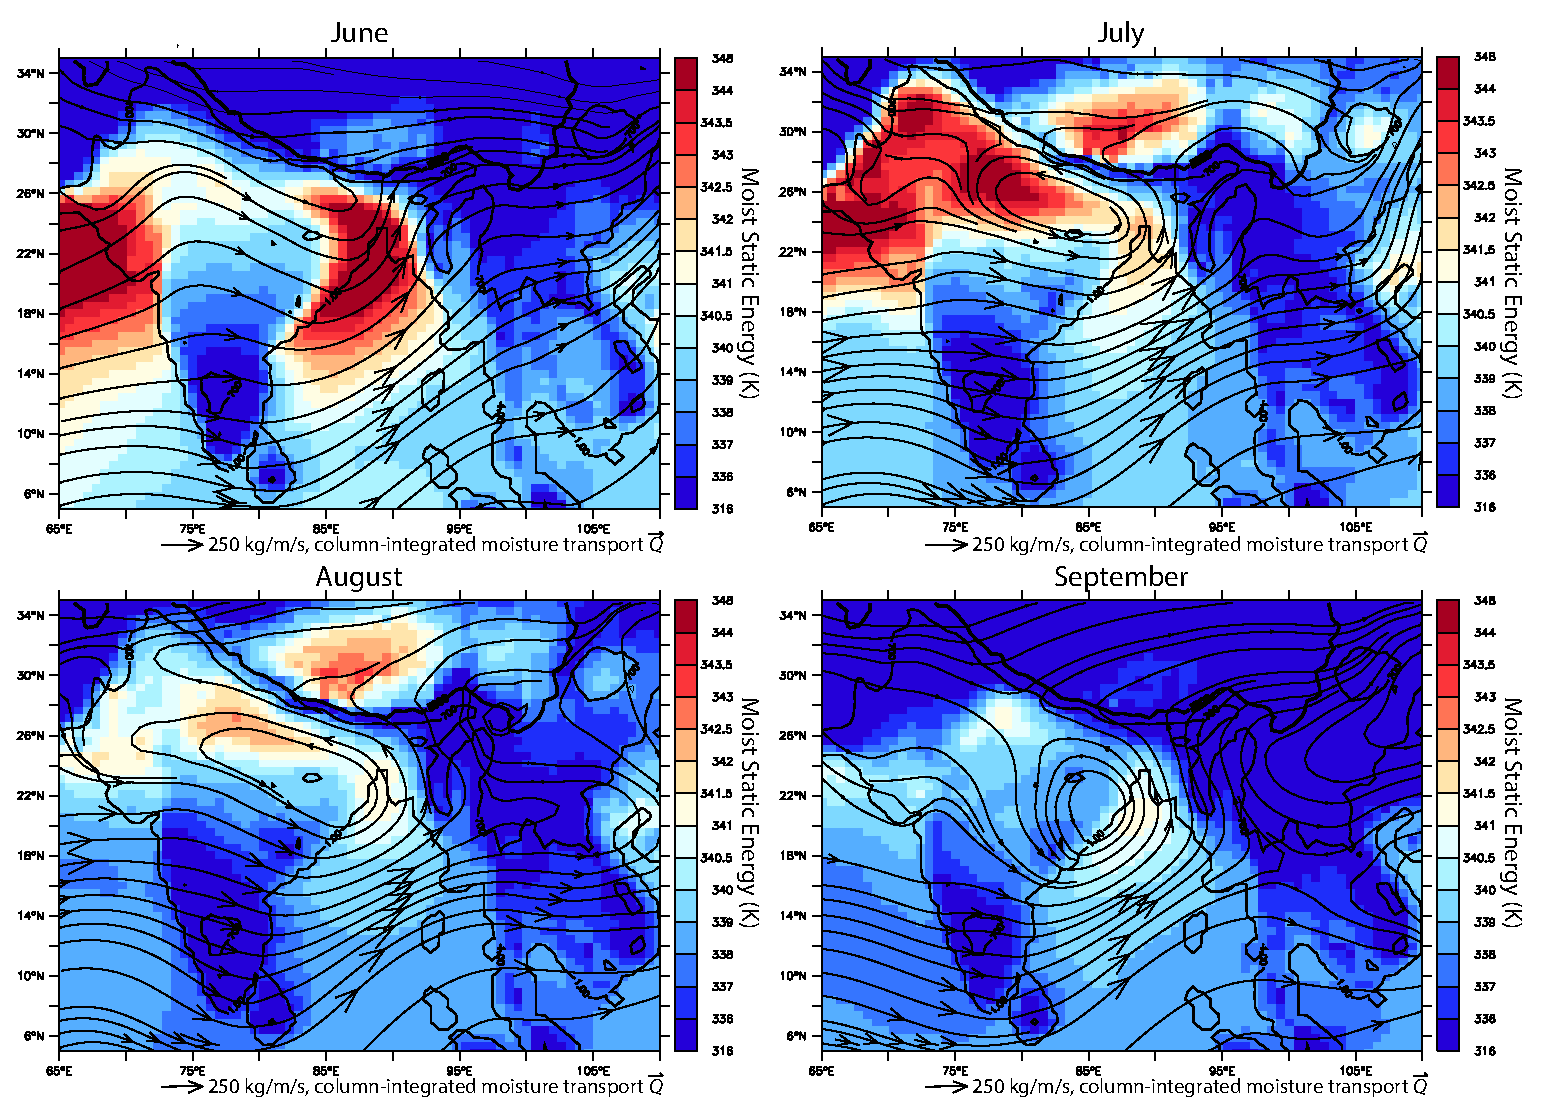
\includegraphics[width=36pc,angle=0]{Figures/ch3/fig11lmdz}\\
  \caption{LMDZ values of near-surface moist static energy $h_b$ (shading) and column-integrated moisture transport $\vec{Q}$ (streamlines, magnitude shown by size of arrowheads) for each month from June to September 2006 over the region 65\textdegree E-110\textdegree E and 5\textdegree N-35\textdegree N. Moist static energy is given by the formula $h_b=c_pT+L_vq+gz$, with specific heat of dry air $c_p$ and latent heat of condensation of water $L_v$, as described in main text. Units of moist static energy are Kelvin, obtained by dividing $h_b$ by $c_p$ as practiced in \cite{Boos2013a}. Column-integrated moisture transport is given by $\vec{Q}=\frac{1}{g}\int q\vec{u}\ \mathrm{d}p $. Note unusual color scale of moist static energy used to emphasize changes over continental India.}
\label{fig:f31}
\end{figure}

